\documentclass[
  captions=tableheading,
  bibliography=totoc, 
  titepage=firstiscover,
]{scrartcl}

\usepackage{blindtext} %neuer input

\usepackage{longtable} % Tabellen über mehrere Seiten

\usepackage[utf8]{inputenc} %neuer input

\usepackage{scrhack}

\usepackage[aux]{rerunfilecheck} %Warnung falls nochmal kompiliert werden muss

\usepackage{fontspec} %Fonteinstellungen

\recalctypearea{}

\usepackage[main=ngerman]{babel} %deutsche Spracheinstellung

\usepackage{ragged2e} %neuer input

\usepackage{amsmath, nccmath}

\usepackage{amssymb} %viele mathe Symbole

\usepackage{mathtools} %Erweiterungen für amsmath


\DeclarePairedDelimiter{\abs}{\lvert}{\rvert}
\DeclarePairedDelimiter{\norm}{\lVert}{\rVert}

\DeclarePairedDelimiter{\bra}{\langle}{\rvert}
\DeclarePairedDelimiter{\ket}{\lvert}{\rangle}

\DeclarePairedDelimiterX{\braket}[2]{\langle}{\rangle}{
#1 \delimsize| #2
}

\NewDocumentCommand \dif {m}
{
\mathinner{\symup{d} #1}
}


\usepackage[
  math-style=ISO,
  bold-style=ISO,
  sans-style=italic,
  nabla=upright,
  partial=upright,
  warnings-off={
    mathtools-colon,
    mathtools-overbracket,
  },
]{unicode-math}

\setmathfont{Latin Modern Math}
\setmathfont{XITS Math}[range={scr, bfscr}]
\setmathfont{XITS Math}[range={cal, bfcal}, StylisticSet=1]


\usepackage[
  locale=DE,
  separate-uncertainty=true,
  per-mode=reciprocal,
  output-decimal-marker={,},
]{siunitx}

\usepackage[autostyle]{csquotes} %richtige Anführungszeichen

\usepackage{xfrac}

\usepackage{float}

\floatplacement{figure}{htbp}

\floatplacement{table}{htbp}

\usepackage[ %floats innerhalb einer section halten
  section,   %floats innerhalb er section halten
  below,     %unterhalb der Section aber auf der selben Seite ist ok
]{placeins}

\usepackage[
  labelfont=bf,
  font=small,
  width=0.9\textwidth,
]{caption}

\usepackage{subcaption} %subfigure, subtable, subref

\usepackage{graphicx}

\usepackage{grffile}

\usepackage{booktabs}

\usepackage{microtype} %Verbesserungen am Schriftbild

\usepackage[
backend=biber,
]{biblatex}

\addbibresource{../lit.bib}

\usepackage[ %Hyperlinks im Dokument
  german,
  unicode,
  pdfusetitle,
  pdfcreator={},
  pdfproducer={},
]{hyperref}

\usepackage{bookmark}

\usepackage[shortcuts]{extdash}

%\usepackage{warpcol}


\begin{document}
    \title{V602 Röntgenemission und -absorption}
    \author{  
    Tobias Rücker\\
    \texorpdfstring{\href{mailto:tobias.ruecker@tu-dortmund.de}{tobias.ruecker@tu-dortmund.de}
    }{}}
    \date{Durchführung: 05.05.2020, Abgabe: 19.05.2020 \vspace{-4ex}}
\maketitle
\thispagestyle{empty}

\newpage
\tableofcontents
\thispagestyle{empty}
\newpage

% Ziel %%%%%%%%%%%%%%%%%%%%%%%%%%%%%%%%%%%%%%%%%%%%%%%%%%%%%%%%%%%%%%%%%%%%%%%%%%%%%%%%%%%%%%%%%%%%%%%%%%%%%%%%%%%%%%%%%%%%%%%%%%%%%%%%%%%%%%%%%%%%%%%%%%%%%%%%%%%%%%%%%%%%%%%%%%%%%%%%%%%%%%%%%%%%%%%%%%%%%%%%%%%%%%%%%

\setcounter{page}{1}
\section{Ziel}\justifying
Absorptionsspektren bilden für die Physik und vor allem für die Astronomie eine entscheidende Rolle
bei der Bestimmung der stofflichen Zusammensetzung wie der Temperatur von strahlenden Himmelskörpern.
Die Kenntnis über die Absorptionsspektren verschiedener Materialien spielt also eine bedeutende
Rolle. Daher werden die Absorptionsspektren verschiedener Materalien mittels einer Röntgenröhre zu
untersucht und deren Abschirmkonstanten bestimmt. 


% Theorie %%%%%%%%%%%%%%%%%%%%%%%%%%%%%%%%%%%%%%%%%%%%%%%%%%%%%%%%%%%%%%%%%%%%%%%%%%%%%%%%%%%%%%%%%%%%%%%%%%%%%%%%%%%%%%%%%%%%%%%%%%%%%%%%%%%%%%%%%%%%%%%%%%%%%%%%%%%%%%%%%%%%%%%%%%%%%%%%%%%%%%%%%%%%%%%%%%

\section{Theorie}\justifying

Zur Untersuchung von Absotptionsspektren werden Röntgenstrahlen verwendet. Diese werden erzeugt, indem
Elektronen aus einer Glühkathode auf eine Anode beschleunigt werden. Das sich ergebende Spektrum 
besteht dabei im wesentlichen aus zwei Bestandteilen. Zum einen existiert ein kontinuierliches Bremsspektrum,
welches aus der Abbremsung der Elektronen entsteht. Diese senden ein Röntgenquant aus, dessen Energie
der verlorenen Energie vom Elektron entspricht. Die Energie des Röntgenquants wird dabei maximal 
bzw. seine Wellelänge minimal, wenn das Elektron vollständig abgebremst wird: \cite{V602}
\begin{align}
\lambda _{\text{min}}=\frac{h \cdot c}{e_0 U} \label{eq:1}
\end{align}
Der andere Teil des Spektrums entsteht durch die charakteristische Strahlung des Anodenmaterials.
Dieses entsteht, wenn ein Elektron ein Atom ionisiert. Dadurch fallen Elektronen von höheren
Schalen auf niedriegere und senden einen Röntgenquant aus, der der Energiedifferenz
der beiden Schalen entspricht \cite{V602}
\begin{align}
    h \nu = E_m - E_n \label{eq:2}
\end{align}
Da die Energieniveaus in Atomen quantisiert bildet das charakteristische Spektrum scharfe Linien.
Die Bezeichnung der einzelnen Linien erfolgt durch $K_{\alpha}, K_{\beta}, L_{\alpha},... $. 
Dabei beschreibt der Buchstabe, auf welcher Schale das Elektron endet und der Index von welchem
es startet.\\
Die einzelnen Linien besitzen bei der Messung jeweils eine gewisse Unschärfe, welche sich durch
\begin{align}
    A=\frac{E_k}{E_{FWHM}} \label{eq:3}
\end{align}
berechnen lässt.
Bei Atomen mit mehreren Elektronen in der Hülle, schwächen diese das Coulombfeld des Atoms ab,
wodurch die Energie eines Elektrons auf der n-ten Schale beschrieben wird durch \cite{V602}
\begin{align}
    E_n = - R_{\infty} z_{\text{eff}}^2 \cdot \frac{1}{n^2} \label{eq:4}, \; R_{\infty}=hR . 
\end{align}
Dabei beschreibt $z_{\text{eff}} =z-\sigma $ die effektive Kernladnug, welche sich aus der 
Kernladungszahl $z$ und der Abschirmkonstante $\sigma$ zusammensetzt. $R_{\infty}=\SI{13.6}{\electronvolt} $ hingegen
beschreibt die Rydbergenrgie und R die Rydberg-Frequenz.
Allerdings lassen sich die Linien der einzelnen Übergänge in eine Feinstruktur aufspalten, wobei die einzelnen
Linien nah beieinander liegen. Beim Anodenspektrum können diese aufgrund der unterliegenden Bremsstrahlung
nicht aufgespaltet werden.\\
Für die Absorption spielen besonders der Photo- und Comptoneffekt bei Röntgenstrahlen, welche kleiner
als $\SI{1}{\mega\electronvolt} $ sind, eine bedeutende Rolle. 
Dabei sinkt der Absorptionskoeffizient mit wachsender Energie, bis die Energie der Photonen
größer als die Bindungsenergie der Elektronen ist. Dann steigt die Funktion sprunghaft an und sinkt danach weiter.
Diese Energie wird Absorptionskante genannt.\\
Die K-Schale besitzt dabei nur eine K-Kante, während die L-Schale durch drei L-Kanten ausgezeichnet ist.
Die Bindungsenergie in der Feinstruktur wird dabei mit der Sommerfeldschen Feinstrukturformel berechnet \cite{V602}
\begin{align}
    E_{n,j}= - R_{\infty} \left(z_{\text{eff},1}^2\cdot \frac{1}{n^2}+\alpha ^2 z_{\text{eff},2}^4\cdot \frac{1}{n^3}\left(\frac{1}{j+\frac{1}{2}}-\frac{3}{4n} \right) \right) \label{eq:5}
\end{align}
\alpha bezeichnet dabei die Sommerfeldsche Feinstrukturkonstante, j der Gesamtdrehimpuls und n 
die Hauptquantenzahl.
MIthilfe der K-Kante und der Formel \eqref{eq:5} lässt sich die Abschirmkonstante für die
K-Schale bestimmen \cite{V602}
\begin{align}
    \sigma _K = Z-\sqrt{\frac{E_K}{R_{\infty}}-\frac{\alpha^2Z^4}{4}} \label{eq:6},
\end{align}
wobei Z die Ordnungszahl ist.\\
Bei der Analyse der Röntgenstrahlung wird diese mit einem LiF-Kristall abhängig von der Wellenlänge in verschiedene
gestreut. Dabei wird die Streuung durch die Bragg'sche Reflexion beschrieben
\begin{align}
    2d \sin \theta =n \lambda \label{eq:7}.
\end{align}

% Versuchsaufbau + Versuchsdurchführung %%%%%%%%%%%%%%%%%%%%%%%%%%%%%%%%%%%%%%%%%%%%%%%%%%%%%%%%%%%%%%%%%%%%%%%%%%%%%%%%%%%%%%%%%%%%%%%%%%%%%%%%%%%%%%%%%%%%%%%%%%%%%%%%%%%%%%%%%%%%%%%%%%%%%%%%%%%%%%%%%%%%%%%%%%%%%%%%%%%%%%%%%%%%%%%%%%

\section{Versuchsaufbau und Versuchsdurchführung}\justifying

Der grundlegende Aufbau besteht aus dem Röntgengerät:\cite{V603}
\begin{figure}[H]
    \centering
    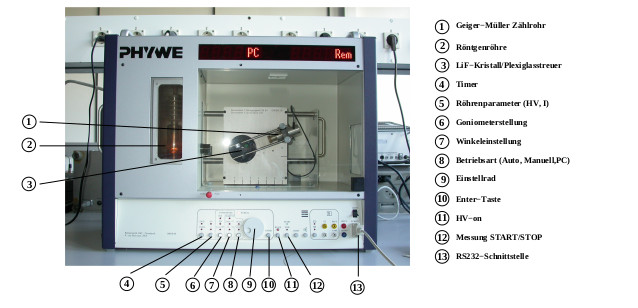
\includegraphics[width=\linewidth]{images/Aufbau1.jpg}
    \caption{Röntgengerät}
    \label{fig:1}
\end{figure}
\flushleft{Alle\;}\justifying Messungen werden dabei über dem Computer gesteuert, dort wird bei dem entsprechenden Programm
das Röntgengerät ausgewählt und Messart, Drehmodus, den anzufahrenden Kristallwinkel und die 
Integrationszeit eingestellt. Die Messart wird auf Spektren gestelltund es wird kontrolliert, ob der
LiF-Kristall und die 1mm Blende in den Halterungen sind und ob die Blende vor dem Geiger-Müllerzählrohr
waagerecht angebracht ist. \\
Für die Überprüfung der Bragg-Bedingung wird der Kristallwinkel auf 14° gestellt und ein Winkelbereich von 26-30°
mit einem Zuwachs von 0,1° eingestellt. Die Integrationszeit wird dabei auf $\SI{5}{\second}$ gestellt.\\
Um das Emissionsspektrum der Anode zu bestimmen, wird eine Integrationszeit von \SI{10}{\second} und
eine Schrittweite von 0,1° eingestellt und eine Messung im passenden Winkelbereich vorgenommen.\\
Für die Messung des Absorptionsspektrum wird jeweils ein Absorber vor das Geiger-Müller Zählrohr positioniert
und eine Messung mit einer Integrationszeit von \SI{20}{\second} und einer Schrittweite von 0,1° durchgeführt werden.
Der Meßbereich sollte dabei angepasst auf das jeweilige Material eingestellt sein. Diese Messung 
wird mit 5 verschiedenen Absorbern mit durchgeführt.

% Auswertung %%%%%%%%%%%%%%%%%%%%%%%%%%%%%%%%%%%%%%%%%%%%%%%%%%%%%%%%%%%%%%%%%%%%%%%%%%%%%%%%%%%%%%%%%%%%%%%%%%%%%%%%%%%%%%%%%%%%%%%%%%%%%%%%%%%%%%%%%%%%%%%%%%%%%%%%%%%%%%%%%%%%%%%%%%%%%%%%%%%%%%%%%%%%%%%%%%

\section{Auswertung}
Alle Messungen sind mit einer Spannung von  \SI{35}{\kilo\volt}, einem Amplitudenstrom von
\SI{1}{\milli\ampere} und einem LiF-Kristall mit einer Gitterkonstanten d von \cite{V602}
\begin{align}
    d = \SI{201.4}{\pico\meter} \label{eq:8}.
\end{align}
Alle Plots in der Auswertung wurden mit Matplotlib \cite{matplotlib} erstellt
und alle Messungenauigkeiten wurden mit uncertainties \cite{uncertainties} berechnet

\subsection{Überprüfung der Bragg'schen Bedingung}
Die Messwerte für die Überprüfung der Bragg'schen Bedingung sind:
\begin{table}
\centering
\caption{Messwerte für die Überprüfung der Bragg'schen Bedingung}
\input{table_Bragg.tex}
\label{tab:1}
\end{table}

\flushleft{Der\;}\justifying aus den Messwerten der Tabelle \ref{tab:1} entstehende PLot sieht
folgendermaßen aus.

\begin{figure}[H]
    \centering
    \includegraphics[width=\linewidth]{build/plot_Bragg.pdf}
    \caption{Lage des Bragg-Peaks \cite{matplotlib}}
    \label{fig:2}
\end{figure}

\flushleft{Der\;}\justifying Plot ist mit curvefit und der Funktion
\begin{subequations}
\begin{align}
    N(\theta) &= A \exp \left(\left(\frac{\theta -B}{C} \right)^2\right)+D \label{eq:9a}
    \intertext{ mit den Parametern
    }
    A&= \text{\input{A_Bragg.tex}},\label{eq:9b} \\
    B&= (\text{\input{B_Bragg.tex}})°,\label{eq:9c} \\
    C&= (\text{\input{C_Bragg.tex}})°\quad \text{und} \label{eq:9d} \\
    D&= \text{\input{D_Bragg.tex}} \label{eq:9e}
\end{align}
\end{subequations}
erstellt worden.\\
Das Maximum der Kurve befindet sich bei 28,15°.
\newpage
\subsection{Emissionsspektrum von Kupfer}

Die Tabelle \ref{tab:1} mit den Messwerten befindet sich im Anhang.

\flushleft{Aus\,}\justifying diesen Messwerten ergibt sich der Graph:
\begin{figure}[H]
    \centering
    \includegraphics[width=\linewidth]{build/plot_Cu.pdf}
    \caption{Emissionsspektrum von Kupfer\cite{matplotlib}} 
    \label{fig:3}
\end{figure}

\flushleft{Die\;}\justifying Maxima der $K_{\alpha} $- und $K_{\beta} $-Linie befinden sich bei:
\begin{subequations}
\begin{align}
    K_{\alpha} &= 22.5°\pm 0.1° \label{10a} \\
    K_{\beta} &= 20.5°\pm 0.1° \label{10b}
\end{align}
\end{subequations}

\flushleft{Um\;}\justifying die Energie zu berechnen, wird die Energie eines Photons 
aus \eqref{eq:2} in Abhängigkeit von der Wellenlänge gesetzt
\begin{align}
    E &= h \nu = h \frac{\omega}{2 \pi}=h \frac{c}{\lambda}. \label{eq:11}\\
    \intertext{
        Nun wird die Bragg'sche Bedingung \eqref{eq:6} für $n=1$ eingesetzt
    }
    E &= \frac{hc}{2d\sin(\theta)} \label{eq:12}.
\end{align}

\flushleft{Damit\;}\justifying werden die Energien für die beiden K-Linien berechnet
\begin{subequations}
\begin{align}
    E_{\alpha} &= \text{\input{E_alpha.tex} }   \label{eq:13a} \\
    E_{\beta} &=   \text{\input{E_beta.tex} } \label{eq:13b} .
\end{align}
\end{subequations}

\flushleft{Die\;}\justifying Halbwertsbreite für die beiden K-Linien ergeben sich aus dem Graphen
\begin{subequations}
\begin{align}
    \Delta E_{FWHM ,\alpha} &=\abs{E(22.85°\pm 0.1°)-E(22.35°\pm 0.1°)} = \text{\input{Delta_E_alpha.tex}} \label{eq:14a} \quad\text{und} \\
    \Delta E_{FWHM ,\beta} &= \abs{E(20.55°\pm 0.1°)-E(20.05°\pm 0.1°) }= \text{\input{Delta_E_beta.tex}} \label{eq:14b}.
\end{align}
\end{subequations}

\flushleft{Die\,}\justifying Auflösung der beiden Spektrallinien wird mit 
den Gleichungen \ref{eq:13a}, \ref{eq:13b}, \ref{eq:14a}, \ref{eq:14b} und \ref{eq:3}
berechnet:
\begin{subequations}
\begin{align}
    A_{\alpha}&= \text{\input{A_alpha.tex}} \label{eq:15a} \\
    A_{\beta}&=  \text{\input{A_beta.tex}} \label{eq:15b}.
\end{align}
\end{subequations}

\flushleft{Für\,}\justifying die Bestimmung der Abschirmkonstante von Kupfer wird Gleichung \eqref{eq:4} verwendet.
Für die Abschirmkonstante $\sigma _1$ wird  diese Gleichung nach $\sigma _1$ umgestellt
\begin{align}
    \sigma_1 &= z-\sqrt{\frac{E_{\text{abs}} }{13.6}}. \label{eq:16}
    \intertext{
        Dabei wird für die Absorptionsenergie der theoretische Literaturwert verwendet  \cite{NIST}.
    Auch die Kernzahl für Kupfer kommt aus dieser Quelle
    }
    E_{\text{abs}}&= \SI{8987.96}{\electronvolt}\label{eq:17}\\
    \sigma _1 &= \text{\input{sigma_1_Cu.tex}} \label{eq:18}.
\end{align}
Für die Abschirmkonstante der beiden K-Strahlen werden die Gleichungen
\eqref{eq:2}, \eqref{eq:4} und \eqref{eq:16}
\begin{align}
    \sigma _{2/3} &= z- \sqrt{\frac{E_{\text{abs}}-E}{13.6} }\cdot 2(\text{bzw}. \cdot 3\, \text{für} \sigma _3)\label{eq:19}\\
    \sigma _2 &= \text{\input{sigma_2.tex}} \label{eq:20} \\
    \sigma _3 &= \text{\input{sigma_3.tex}} \label{eq:21}.
\end{align}

\flushleft{Die\,}\justifying theoretischen Werte der Abschirmkonstanten werden mit den theoretischen
Werten \cite{NIST} für die $K_{\alpha} $- und $K_{\beta} $-Linie berechnet:
\begin{align}
    E_{\alpha, \text{theo}}&= \SI{8048.11}{\electronvolt} \label{eq:22} \\
    E_{\beta, \text{theo}}&= \SI{8906.9}{\electronvolt}. \label{eq:23}\\
    \sigma _{2,\text{theo}} &=  \text{\input{sigma_2_theo.tex}} \label{eq:24} \\
    \sigma _{3,\text{theo}} &=  \text{\input{sigma_3_theo.tex}} \label{eq:25}.
\end{align}


\subsection{Untersuchung der Absorptionsspektren}

Für die verschiedenen Elemente werden jeweils zuerst die Tabellen
mit den Messwerten dargestellt und dann werden die Graphen
dargestellt. In den Graphen werden jeweils das Minimum und das Maximum
der K-Kante dargestellt.
Danach wird die Intensität in der Mitte der Kante über die Formel \cite{V602}
\begin{align}
    I_k = I_K^{\text{min}}+\frac{I_K^{\text{max}}-I_K^{\text{min}}}{2} \label{eq:26}
\end{align}
bestimmt.
Danach wird der jeweilige Winkel zur Intensität aus dem Graphen bestimmt und damit
die Absorptionsenergie wie zuvor schon bestimmt. \\
Aus der Absorptionsenergie wird mit der Gleichung \eqref{eq:6} die Abschirmkonstante berechnet.
Die Sommerfeldsche Konstante wird dabei aus der Quelle \cite{ertel1935sommerfeldsche}
entnommen
Zuletzt wird mit den Theoriewerten für die Energie, welche aus der Quelle \cite{NIST}
stammen, die theoretischen Abschirmkonstanten berechnet.

\flushleft{Den\,}\justifying Anfang macht der Absorber aus Brom.
\input{build/table_Br.tex}

\begin{figure}[H]
    \centering
    \includegraphics[width=\linewidth]{build/plot_Br.pdf}
    \caption{Absorptionsspektrum von Brom\cite{matplotlib}}
    \label{fig:4}
\end{figure}

\flushleft{Das\,}\justifying Intensitätsmaximum und -minimum für Brom liegen bei 13° und 13,5°.
Dadurch liegt die Mitte der Intensität bei $(13,2\pm 0,1)°$.
Die Energie und die Abschirmkonstante ergeben
\begin{align}
    E_{\text{Br}}&= \text{\input{E_Brom.tex} }  \label{eq:27} \\
    \sigma_{\text{Br}}&= \text{\input{sigma_Brom.tex} }  \label{eq:28}.
\end{align}
Der theoretische Wert beträgt 
\begin{align}
    \sigma_{\text{Br,theo.}}&= \text{\input{sigma_Brom_theo.tex} }  \label{eq:29}
\end{align}
mit einem Energiewert von \SI{13483.86}{\electronvolt} \cite{NIST} .

\flushleft{Nun\,}\justifying geht es weiter mit dem Galliumabsorber.
\input{build/table_Ga.tex}

\begin{figure}[H]
    \centering
    \includegraphics[width=\linewidth]{build/plot_Ga.pdf}
    \caption{Absorptionsspektrum von Gallium\cite{matplotlib}}
    \label{fig:5}
\end{figure}

\flushleft{Für\,}\justifying Gallium befindet sich das Intensitätsmaximum und -minimum
bei 17,8° und 17,1°. Die Mitte der Intensität
findet sich im Graph dadurch bei $(17,35\pm 0,1)°$.
Für die Abschirmkonstante und die Energie ergeben sich daher
\begin{align}
    E_{\text{Ga}}&= \text{\input{E_Gallium.tex}} \label{eq:30}\\
    \sigma _{\text{Ga}} &= \text{\input{sigma_Gallium.tex}} \label{eq:31}.
\end{align}
Für die theoretische Abschirmkonstante ergibt sich 
mit einer Energie von $\SI{10377.76}{\electronvolt} $ \cite{NIST} eine 
Abschirmkonstante von
\begin{align}
    \sigma _{\text{Ga,theo.}} = \text{\input{sigma_Gallium_theo.tex}} \label{eq:32}.
\end{align}


\flushleft{Jetzt\,}\justifying kommt die Auswertung des Absorbers aus Rubidium.
\input{build/table_Rb.tex}

\begin{figure}[H]
    \centering
    \includegraphics[width=\linewidth]{build/plot_Rb.pdf}
    \caption{Absorptionsspektrum von Rubidium\cite{matplotlib}}
    \label{fig:6}
\end{figure}

\flushleft{Hier\,}\justifying bei Rubidium sind das Intensitätsmaximum und -minimum bei 12,1° und 11,4° zu finden.
Für die Mitte der Intensität ergibt sich dadurch ein Wert von $(11,77 \pm 0.1)° $.
Dadurch betragen Abschirmkonstante und Energie die Werte
\begin{align}
    E_{\text{Rb}}&= \text{\input{E_Rb.tex}} \label{eq:33}\\
    \sigma _{\text{Rb}} &= \text{\input{sigma_Rb.tex}} \label{eq:34}.
\end{align}
Der theoretische Wert für die Abschirmkonstante hingegen hat den Wert
\begin{align}
    \sigma _{\text{Rb,theo.}}=\text{\input{sigma_Rb_theo}} \label{eq:35},
\end{align}
wobei die Energie $\SI{15207.74}{\electronvolt}$ \cite{NIST} ist.

\flushleft{Als\,}\justifying nächstes wird der Strontium-Absorber ausgewertet.
\input{build/table_Sr.tex}

\begin{figure}[H]
    \centering
    \includegraphics[width=\linewidth]{build/plot_Sr.pdf}
    \caption{Absorptionsspektrum von Strontium\cite{matplotlib}}
    \label{fig:7}
\end{figure}
\flushleft{Bei\,}\justifying dem Graphe des Strontium-Absorbers finden sich das Intensitätsmaximum
und -minimum der K-Kante bei den Werten 11,4° und 10,7°.
Die Mitte der K-Kante befindet sich bei $(11,08\pm0,1)° $.
Für die Energie und die Abschirmkonstante ergibt sich dadurch
\begin{align}
    E_{\text{Sr}}&= \text{\input{E_Sr}} \label{eq:36}\\
    \sigma _{\text{Sr}} &= \text{\input{sigma_Sr.tex}} \label{eq:37}.
\end{align}
Im Vergleich dazu beträgt der theoretische Wert  mit einer Energie von $\SI{16115.26}{\electronvolt} $ \cite{NIST}
\begin{align}
    \sigma _{\text{Sr,theo.}} &= \text{\input{sigma_Sr_theo.tex}} \label{eq:38}.
\end{align}


\flushleft{Nun\,}\justifying wird das ganze für den Zink-Absorber angewendet.
\input{build/table_Zn.tex}

\begin{figure}[H]
    \centering
    \includegraphics[width=\linewidth]{build/plot_Zn.pdf}
    \caption{Absorptionsspektrum von Zink\cite{matplotlib}}
    \label{fig:8}
\end{figure}

\flushleft{Aus}\justifying der Graphik und den Messwerten lässt sich das Intensitätsmaxium und 
-minimum bei 19,0° und 18,4° bestimmen.
Die Mitte der K-Kante kann bei $(18,65\pm 0,1)° $ lokalisiert werden.
Für die Absorptionsenergie und die Abschirmkonstante bedeutet das einen Wert von
\begin{align}
    E_{\text{Zn}} &= \text{\input{E_Zn.tex}} \label{eq:39}\\
    \sigma _{\text{Zn}} &= \text{\input{sigma_Zn.tex}} \label{eq:40}.
\end{align}
Mit einer Absorptionsenergie von $\SI{9668.55}{\electronvolt} $ \cite{NIST} errechnet
sich für die Absorptionskonstante ein Wert von
\begin{align}
    \sigma _{\text{Zn,theo.}}&= \text{\input{sigma_Zn_theo.tex}} \label{eq:41}.
\end{align}


\flushleft{Zu\,}\justifying guter letzt wird noch Zirkonium ausgewertet.
\input{build/table_Zr.tex}

\begin{figure}[H]
    \centering
    \includegraphics[width=\linewidth]{build/plot_Zr.pdf}
    \caption{Absorptionsspektrum von Zirkonium\cite{matplotlib}}
    \label{fig:9}
\end{figure}
\flushleft{Bei\,}\justifying Zirkonium ergeben sich für das Intensitätsmaximum und -minimum
10,4° und 9,5°.
Die Mitte der K-Kante befindet sich dementsprechend bei $(9,95\pm 0,1)°$.
Für die Absorptionsenergie und die Abschirmkonstante ergeben sich daher
die Werte
\begin{align}
    E_{\text{Zr}} &= \text{\input{E_Zr.tex}} \label{eq:42} \\
    \sigma _{\text{Zr}} &= \text{\input{sigma_Zr.tex}} \label{eq:43}.
\end{align}
Für den theoretischen Wert gibt das entsprechend
\begin{align}
    \sigma _{\text{Zr,theo.}} = \text{\input{sigma_Zr_theo.tex}} \label{eq:44}
\end{align}
mit einer Energie von $\SI{18008.15}{\electronvolt} $ \cite{NIST}.


\flushleft{Mithilfe\,}\justifying der einzelnen Absorptionsenergien, den Kernzahlen und den Abschirmkonstanten
lässt sich die Relation \cite{V602}
\begin{align}
    E_k &= hR (z-\sigma)^2 \label{eq:45}\\
    \sqrt{E_k}&=\sqrt{hR} (z_{\text{eff}} ) \label{eq:46}
\end{align}
zeigen.\\
Der Graph sieht dabei wie folgt aus:
\begin{figure}[H]
    \centering
    \includegraphics[width=\linewidth]{build/plot_Ez.pdf}
    \caption{ Diagramm\cite{matplotlib}}
    \label{fig:10}
\end{figure}
Die Parameter der Ausgleichsgeraden sind mit der Funktion polyftit aus Scipy erstellt
worden und lauten
\begin{align}
    a &= \text{\input{a.tex}} \label{eq:47} \\
    b &= \text{\input{b.tex}} \label{eq:48}.
\end{align}
Die Theoriekurve wurde der Wert für $R_{\infty}=hR=\SI{13.6}{\electronvolt} $ in 
Gleichung \eqref{eq:45} eingesetzt und geplottet.\\
Aus der Steigung a lässt sich die Rydbergfrequenz R berechnen
\begin{align}
    R&=\frac{a^2}{h} \label{eq:49}\\
    R&= \text{\input{R.tex}} \label{eq:50}\\
    R_{\text{theo}}&= \text{\input{R_theo.tex}} \label{eq:51}.
\end{align}

% Diskussion %%%%%%%%%%%%%%%%%%%%%%%%%%%%%%%%%%%%%%%%%%%%%%%%%%%%%%%%%%%%%%%%%%%%%%%%%%%%%%%%%%%%%%%%%%%%%%%%%%%%%%%%%%%%%%%%%%%%%%%%%%%%%%%%%%%%%%%%%%%%%%%%%%%%%%%%%%%%%%%%%%%%%%%%%%%%%%%%%%%%%%%%%%%%%%%%%%

\section{Diskussion}

In der nachfolgenden Tabelle finden sich alle zur Diskussion notwendigen Werte
mitsamt ihrer Literaturwerte und der relativen Fehler aufgetragen.

\begin{table}[H]
\centering
\caption{Messwerte, Literaturwerte und ihre relativen Fehler}
\begin{tabular}{c c c c}
    \toprule
    \multicolumn{2}{c}{Messwert} &\multicolumn{1}{c}{Literatur-/theo. Wert}  &\multicolumn{1}{c}{Relativer Fehler $\frac{mess-lit}{lit} $}  \\
    \cmidrule(lr){1-4} 
       $\theta _{\text{max,Bragg}}$ & 28,15°  & 28° & \text{\input{relerr_max.tex}}\% \\
       $E_{K_{\alpha}} $ & \text{\input{E_alpha.tex}} & \SI{8048.11}{\electronvolt} \cite{NIST} & \text{\input{relerr_E_alpha.tex}}\% \\
       $E_{K_{\beta}}$ & \text{\input{E_beta.tex}} & \SI{8906.9}{\electronvolt}\cite{NIST} & \text{\input{relerr_E_beta.tex}}\%  \\
       $A_{\alpha} $ & \text{\input{A_alpha.tex}} & - & - \\
       $A_{\beta} $ & \text{\input{A_beta.tex}} & - & - \\
       $\sigma _1 $ & - & \text{\input{sigma_1_Cu.tex}} & - \\
       $\sigma _2 $ & \text{\input{sigma_2.tex}} & 12,37 & \text{\input{relerr_sigma_alpha.tex}} \% \\
       $\sigma _3 $ & \text{\input{sigma_3.tex}} & 21,68 & \text{\input{relerr_sigma_beta.tex}}\% \\
       $E_{Br} $ & \text{\input{E_Brom.tex}} & \SI{13483.86}{\electronvolt}\cite{NIST} & \text{\input{relerr_E_Brom.tex}}\%  \\
       $\sigma _{Br} $ & \text{\input{sigma_Brom.tex}} & \text{\input{sigma_Brom_theo.tex}} & \text{\input{relerr_sigma_Brom.tex}}\% \\
       $E_{Ga}$ & \text{\input{E_Gallium.tex}} & \SI{10377.76}{\electronvolt}\cite{NIST} & \text{\input{relerr_sigma_Gallium.tex}}\% \\
       $\sigma _{Ga} $ & \text{\input{sigma_Gallium.tex}} & \text{\input{sigma_Gallium_theo.tex}} & \text{\input{relerr_sigma_Gallium.tex}}\% \\
       $E_{Rb}$ & \text{\input{E_Rb.tex}} & \SI{15207.74}{\electronvolt}\cite{NIST} & \text{\input{relerr_E_Rb.tex}} \%\\
       $\sigma _{Rb} $ & \text{\input{sigma_Rb.tex}} & \text{\input{sigma_Rb_theo.tex}} & \text{\input{relerr_sigma_Rb.tex}} \%\\
       $E_{Sr}$ & \text{\input{E_Sr.tex}} & \SI{16115.26}{\electronvolt}\cite{NIST} & \text{\input{relerr_E_Sr.tex}}\% \\
       $\sigma _{Sr} $ & \text{\input{sigma_Sr.tex}} & \text{\input{sigma_Sr_theo.tex}} & \text{\input{relerr_sigma_Sr.tex}}\% \\
       $E_{Zn}$ & \text{\input{E_Zn.tex}} & \SI{9668.55}{\electronvolt}\cite{NIST} & \text{\input{relerr_E_Zn.tex}}\% \\
       $\sigma _{Zn} $ & \text{\input{sigma_Zn.tex}} & \text{\input{sigma_Zn_theo.tex}} & \text{\input{relerr_sigma_Zn.tex}} \%\\
       $E_{Zr}$ & \text{\input{E_Zr.tex}} & \SI{18008.15}{\electronvolt}\cite{NIST} & \text{\input{relerr_E_Zr.tex}}\% \\
       $\sigma _{Zr} $ & \text{\input{sigma_Zr.tex}} & \text{\input{sigma_Zr_theo.tex}} & \text{\input{relerr_sigma_Zr.tex}} \%\\
       $R$ & \text{\input{R.tex}} & \text{\input{R_theo.tex}} & \text{\input{relerr_R.tex}}\% \\
    \bottomrule
\end{tabular}
\label{tab:9}
\end{table}

\flushleft{Bei\,}\justifying der Überprüfung der Bragg-Bedingung ist das Maximum bei einem Winkel von 28,15° ermittelt worden.
Das stimmt mit dem ziemlich genau mit dem theoretischen Wert von 28° überein. Den theoretischen Bragg-
Winkel wird durch die Verdopplung des eingestellten Kristallwinkels erhalten.
Für die Messungen ist es von besonderer Bedeutung, dass die Bragg-Bedingung erfüllt
ist, da selbst eine kleine Abweichung von 3° alle Messungen verfälschen könnte.\\

\flushleft{Bei\,}\justifying den Energien für das Emissionsspektrum von Kupfer zeigen sich sehr geringe relative Fehler
auf, was bedeutet, dass das Spektrum bei der Messung in keiner Form verfälscht ist.
Das Auflösevermögen der einzelnen charakteristischen Linie zeigt allerdings eine
Messungenauigkeit im gleichen Größenbereich  auf. Dadurch ist es scwer zu sagen,
wie zuverlässig diese Angabe ist. Der hohe Fehler könnte durch den sehr großen 
Messbereich stammen, wodurch die genaue Bestimmung der Halbwertsbreite nicht
einfach ist. Auch der vorliegende Untergrund durch die Bremsstrahlung 
verschiebt die eigentliche Halbwertsbreite, wodurch sie kaum
aussagekräftig ist.\\ 
Die Abschirmkonstanten von Kupfer in der Tabelle \ref{tab:9} für die $K_{\alpha}- $
und $K_{\beta} $-Linie zeigen im Vergleich zu den Literaturwerten nur geringe relative
Fehler auf. Die Literaturwerte liegen dabei innerhalb der jeweiligen Fehlerintervalle.
Die Messung der Absorptionskante konnte dabei nicht mit der vorliegenden Apparatur
bestimmt werden, weshalb zu Berechnung der anderen beiden Abschirmkonstante der 
Literaturwert verwendet worden ist.\\
Die einzelnen Absorptionsenergien und Abschirmkonstanten der verschiedenen haben
realtiv geringe Fehler un bei den meistens liegen die Literaturwerte innerhalb
der Fehlergrenzen der einzelnen Werte. Die existierenden Fehler können 
statistische Fehler sein. Zudem ist bei der Auswertung mit der Bragg-
Bedingun nur die 1. Ordnung betrachtet worden, was zusätzliche
Strahlung höherer Ordnung damit nicht einbezogen hat.
Der höchste Fehler unter diesen
liegt bei der Aschirmkonstante von Zirkonium vor mit 4,88\%. \\
Die Besimmung der Rydbergfrequenz hat ebenso eine relativ geringe Abweichung,
womit das Moseleysche Gesetz \eqref{eq:45} bestätigt wird. Der vorhandene
Fehler ensteht durch die bereits vorhandenen Fehler der einzelnen Energien und
hängt direkt mit deren Fehlern zusammen.


% Literatur %%%%%%%%%%%%%%%%%%%%%%%%%%%%%%%%%%%%%%%%%%%%%%%%%%%%%%%%%%%%%%%%%%%%%%%%%%%%%%%%%%%%%%%%%%%%%%%%%%%%%%%%%%%%%%%%%%%%%%%%%%%%%%%%%%%%%%%%%%%%%%%%%%%%%%%%%%%%%%%%%%%%%%%%%%%%%%%%%%%%%%%%%%%%%%%%%%

\newpage
\printbibliography
\newpage
\section{Anhang}
\input{table_Cu.tex}
\end{document}